% Stat 794: Knitr lab
% Illustrating knitr to present analyses of College data from ISLR text
% Packages required: knitr, xtable, stargazer, ISLR
% To use, make sure to call library(knitr) first in console
% To run and create a .tex file: knit('knitr_lab_ClassVersion.Rnw') in R

% To show at start of class:
% -- Step through preface briefly and show where to enter name
% -- LaTeX preface (preface.tex) vs. Knitr preface (knitr_ClassVersion.Rnw);
%    briefly delineate two approaches to report writing
% -- Code in place for regression analysis and prediction
% -- There are 6 tasks to complete with sample code and hints where needed
% -- Suggest cutting an pasting R code into console first to debug
% -- Tasks 1, 2, 4, and 5 ask you to compose text discussing the output 
%    for that task.


% Preface required in the knitr RnW file
\documentclass{article}\usepackage[]{graphicx}\usepackage[]{color}
% maxwidth is the original width if it is less than linewidth
% otherwise use linewidth (to make sure the graphics do not exceed the margin)
\makeatletter
\def\maxwidth{ %
  \ifdim\Gin@nat@width>\linewidth
    \linewidth
  \else
    \Gin@nat@width
  \fi
}
\makeatother

\definecolor{fgcolor}{rgb}{0.345, 0.345, 0.345}
\newcommand{\hlnum}[1]{\textcolor[rgb]{0.686,0.059,0.569}{#1}}%
\newcommand{\hlstr}[1]{\textcolor[rgb]{0.192,0.494,0.8}{#1}}%
\newcommand{\hlcom}[1]{\textcolor[rgb]{0.678,0.584,0.686}{\textit{#1}}}%
\newcommand{\hlopt}[1]{\textcolor[rgb]{0,0,0}{#1}}%
\newcommand{\hlstd}[1]{\textcolor[rgb]{0.345,0.345,0.345}{#1}}%
\newcommand{\hlkwa}[1]{\textcolor[rgb]{0.161,0.373,0.58}{\textbf{#1}}}%
\newcommand{\hlkwb}[1]{\textcolor[rgb]{0.69,0.353,0.396}{#1}}%
\newcommand{\hlkwc}[1]{\textcolor[rgb]{0.333,0.667,0.333}{#1}}%
\newcommand{\hlkwd}[1]{\textcolor[rgb]{0.737,0.353,0.396}{\textbf{#1}}}%
\let\hlipl\hlkwb

\usepackage{framed}
\makeatletter
\newenvironment{kframe}{%
 \def\at@end@of@kframe{}%
 \ifinner\ifhmode%
  \def\at@end@of@kframe{\end{minipage}}%
  \begin{minipage}{\columnwidth}%
 \fi\fi%
 \def\FrameCommand##1{\hskip\@totalleftmargin \hskip-\fboxsep
 \colorbox{shadecolor}{##1}\hskip-\fboxsep
     % There is no \\@totalrightmargin, so:
     \hskip-\linewidth \hskip-\@totalleftmargin \hskip\columnwidth}%
 \MakeFramed {\advance\hsize-\width
   \@totalleftmargin\z@ \linewidth\hsize
   \@setminipage}}%
 {\par\unskip\endMakeFramed%
 \at@end@of@kframe}
\makeatother

\definecolor{shadecolor}{rgb}{.97, .97, .97}
\definecolor{messagecolor}{rgb}{0, 0, 0}
\definecolor{warningcolor}{rgb}{1, 0, 1}
\definecolor{errorcolor}{rgb}{1, 0, 0}
\newenvironment{knitrout}{}{} % an empty environment to be redefined in TeX

\usepackage{alltt}

\usepackage{rotating}
\usepackage{graphics}
\usepackage{latexsym}
\usepackage{color}
\usepackage{listings} % allows for importing code scripts into the tex file
\usepackage{dcolumn}

% Approximately 1 inch borders all around
\setlength\topmargin{-.56in}
\setlength\evensidemargin{0in}
\setlength\oddsidemargin{0in}
\setlength\textwidth{6.49in}
\setlength\textheight{8.6in}

% Options for code listing; from Patrick DeJesus, October 2016
\definecolor{codegreen}{rgb}{0,0.6,0}
\definecolor{codegray}{rgb}{0.5,0.5,0.5}
\definecolor{codepurple}{rgb}{0.58,0,0.82}
\definecolor{backcolour}{rgb}{0.95,0.95,0.92}
\lstdefinestyle{mystyle}{
	backgroundcolor=\color{backcolour},   commentstyle=\color{codegreen},
	keywordstyle=\color{magenta},
	numberstyle=\tiny\color{codegray},
	stringstyle=\color{codepurple},
	basicstyle=\footnotesize,
	breakatwhitespace=false,         
	breaklines=true,                 
	captionpos=b,                    
	keepspaces=true,                 
	numbers=left,                    
	numbersep=5pt,                  
	showspaces=false,                
	showstringspaces=false,
	showtabs=false,                  
	tabsize=2
}
%"mystyle" code listing set
\lstset{style=mystyle}
%\lstset{inputpath=appendix/}


\title{Stat 794, Example Application of \texttt{knitr}} 
\author{Kristine Dinh}
\date{\today}
\IfFileExists{upquote.sty}{\usepackage{upquote}}{}
\begin{document} 
\maketitle

% Code to start knitr


%%%%%%%%%%%%%%%%%%%%%%%%%%%%%%%%%%%%%%%%%%%%%%%%%%%%%%%%%%%%
% Code snippet to load in libraries and data  
% THIS IS HOW R-CODE IS READ INTO LaTeX DOC WITH knitr
% Environment:  
% <<...>>=  
% [Code here] 
% @
%%%%%%%%%%%%%%%%%%%%%%%%%%%%%%%%%%%%%%%%%%%%%%%%%%%%%%%%%%%%


  
% Code snippet to run the regression analysis, including prediction for two new Universities



%%%%%%%%%%%%%%
% Lab Tasks
%%%%%%%%%%%%%%

%% Task 1: Present an R dump of the summary of the regression fit
% [Place knitr code chunk here]
\begin{knitrout}
\definecolor{shadecolor}{rgb}{0.969, 0.969, 0.969}\color{fgcolor}\begin{kframe}
\begin{alltt}
\hlkwd{stargazer}\hlstd{(fm1,} \hlkwc{title} \hlstd{=} \hlstr{"Summary of Regression"}\hlstd{)}
\end{alltt}
\begin{verbatim}
## 
## % Table created by stargazer v.5.2.2 by Marek Hlavac, Harvard University. E-mail: hlavac at fas.harvard.edu
## % Date and time: Thu, Sep 03, 2020 - 11:04:15 AM
## \begin{table}[!htbp] \centering 
##   \caption{Summary of Regression} 
##   \label{} 
## \begin{tabular}{@{\extracolsep{5pt}}lc} 
## \\[-1.8ex]\hline 
## \hline \\[-1.8ex] 
##  & \multicolumn{1}{c}{\textit{Dependent variable:}} \\ 
## \cline{2-2} 
## \\[-1.8ex] & Apps \\ 
## \hline \\[-1.8ex] 
##  PrivateYes & $-$291.623$^{**}$ \\ 
##   & (133.283) \\ 
##   & \\ 
##  EliteYes & 1,745.002$^{***}$ \\ 
##   & (151.741) \\ 
##   & \\ 
##  Accept & 1.429$^{***}$ \\ 
##   & (0.020) \\ 
##   & \\ 
##  Outstate & $-$0.014 \\ 
##   & (0.017) \\ 
##   & \\ 
##  Room.Board & 0.166$^{***}$ \\ 
##   & (0.050) \\ 
##   & \\ 
##  Grad.Rate & 8.635$^{***}$ \\ 
##   & (2.947) \\ 
##   & \\ 
##  Constant & $-$985.954$^{***}$ \\ 
##   & (204.824) \\ 
##   & \\ 
## \hline \\[-1.8ex] 
## Observations & 777 \\ 
## R$^{2}$ & 0.916 \\ 
## Adjusted R$^{2}$ & 0.915 \\ 
## Residual Std. Error & 1,128.032 (df = 770) \\ 
## F Statistic & 1,394.089$^{***}$ (df = 6; 770) \\ 
## \hline 
## \hline \\[-1.8ex] 
## \textit{Note:}  & \multicolumn{1}{r}{$^{*}$p$<$0.1; $^{**}$p$<$0.05; $^{***}$p$<$0.01} \\ 
## \end{tabular} 
## \end{table}
\end{verbatim}
\end{kframe}
\end{knitrout}

% ... allows us to run R-code or grab R elements inside the text.
% Try it out!  Write a sentence using \Sexpr to grab the predicted values for 
% the new schools (variables newpred1 and newpred2 from above).
Predicted values for the new schools are: 7000, 4800, 9300 and 2300, 57, 4600 

%% Task 2: Insert a pairwise scatterplot into your document
% For plots, start by setting up the LaTeX figure environment,
% then place R code to knit, then set up LaTeX code to complete figure environment.
% Below I give the code for this task.  You will practice with this code in Task 5.
\begin{figure}
\begin{center}
\begin{knitrout}
\definecolor{shadecolor}{rgb}{0.969, 0.969, 0.969}\color{fgcolor}
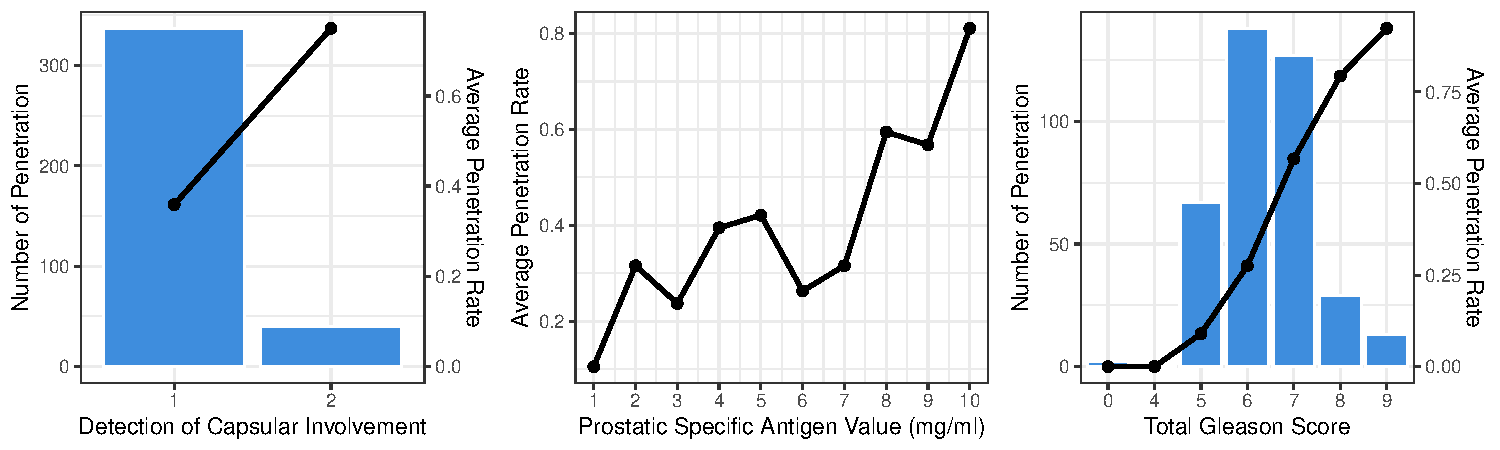
\includegraphics[width=4in]{figure/unnamed-chunk-2-1} 

\end{knitrout}
\caption{Pairwise scatterplot of variables}
\label{pairwise_scatterplot}
\end{center}
\end{figure}

% Write a short blurb of text to cite your figure.  To cite use the \ref function an call the label assigned: Figure~\ref{pairs}.
When exploring the relationship between each variable, a pairwise scatterplot was created, see Figure~\{pairwise_scatterplot}. As seen in plot, Outstate and Room Board are highly correlated. 


%% Task 3: Use stargazer to present summary statistics of the College data set

% Table created by stargazer v.5.2.2 by Marek Hlavac, Harvard University. E-mail: hlavac at fas.harvard.edu
% Date and time: Thu, Sep 03, 2020 - 11:04:15 AM
% Requires LaTeX packages: rotating 
\begin{sidewaystable}[!htbp] \centering 
  \caption{Summary statistics for the ISLR College data set.} 
  \label{descrips} 
\begin{tabular}{@{\extracolsep{5pt}}lccccccc} 
\\[-1.8ex]\hline 
\hline \\[-1.8ex] 
Statistic & \multicolumn{1}{c}{Mean} & \multicolumn{1}{c}{Median} & \multicolumn{1}{c}{St. Dev.} & \multicolumn{1}{c}{Min} & \multicolumn{1}{c}{Pctl(25)} & \multicolumn{1}{c}{Pctl(75)} & \multicolumn{1}{c}{Max} \\ 
\hline \\[-1.8ex] 
Private Flag & 3,001.638 & 1,558 & 3,870.201 & 81 & 776 & 3,624 & 48,094 \\ 
Application Count & 2,018.804 & 1,110 & 2,451.114 & 72 & 604 & 2,424 & 26,330 \\ 
Acceptance Count & 779.973 & 434 & 929.176 & 35 & 242 & 902 & 6,392 \\ 
Enrollment Count & 27.559 & 23 & 17.640 & 1 & 15 & 35 & 96 \\ 
Top 10 Percent in High School & 55.797 & 54 & 19.805 & 9 & 41 & 69 & 100 \\ 
Top 25 Percent in High School & 3,699.907 & 1,707 & 4,850.421 & 139 & 992 & 4,005 & 31,643 \\ 
Full-time Undergrad & 855.299 & 353 & 1,522.432 & 1 & 95 & 967 & 21,836 \\ 
Part-time Undergrad & 10,440.670 & 9,990 & 4,023.016 & 2,340 & 7,320 & 12,925 & 21,700 \\ 
Out-of-state tuition & 4,357.526 & 4,200 & 1,096.696 & 1,780 & 3,597 & 5,050 & 8,124 \\ 
Room and board Costs & 549.381 & 500 & 165.105 & 96 & 470 & 600 & 2,340 \\ 
Estimated Book Costs & 1,340.642 & 1,200 & 677.071 & 250 & 850 & 1,700 & 6,800 \\ 
Estimated Personal Costs & 72.660 & 75 & 16.328 & 8 & 62 & 85 & 103 \\ 
Percent of Faculty with PhD & 79.703 & 82 & 14.722 & 24 & 71 & 92 & 100 \\ 
Percent of Faculty with termianl Degree & 14.090 & 13.600 & 3.958 & 2.500 & 11.500 & 16.500 & 39.800 \\ 
Student/Faculty Ratio & 22.744 & 21 & 12.392 & 0 & 13 & 31 & 64 \\ 
Percent of alumni donated & 9,660.171 & 8,377 & 5,221.768 & 3,186 & 6,751 & 10,830 & 56,233 \\ 
Instructional expenditure per student & 65.463 & 65 & 17.178 & 10 & 53 & 78 & 118 \\ 
\hline \\[-1.8ex] 
\end{tabular} 
\end{sidewaystable} 



%% Task 4: Create a table of predictions using xtable
% I provide the code below for a base table.  
% The task is then to add additional columns to the table and create the LaTeX code using xtable.
% Note that we use results="asis" to force knitr to present the table code for compiling in LaTeX
% latex table generated in R 3.6.2 by xtable 1.8-4 package
% Thu Sep 03 11:04:16 2020
\begin{table}[ht]
\centering
\begin{tabular}{|l|rrrrrrr|}
  \hline
 & univ & elite & gradrate & preds & lwr & upr & outstate \\ 
  \hline
1 & University 1 & No & 0.60 & 7000.00 & 4800.00 & 9300.00 & 8000.00 \\ 
  2 & University 2 & Yes & 0.90 & 2300.00 & 57.00 & 4600.00 & 16000.00 \\ 
   \hline
\end{tabular}
\caption{Prediction Table} 
\label{pred_table}
\end{table}


% Write a short blurb citing your tables.  As with figures, to cite this table use the \ref function and call the label assigned: Table~\ref{desrips2} for the descriptive statistics table and Table~\ref{modelinf} for the inference table.
As seen in Table~\ref{pred_table}, University 1 recieved more applications than University 2. 



%% Task 5: Create an appendix of plots
% We will create a 2x2 graphic of regression diagnostics
\newpage
\noindent \Large{{\bf Appendix A: Supplementary Plots}}
\begin{figure}[h!]
\begin{center}
%%%%%%%%%%%%%%%%
% Here is code for the default regression diagnostics from R
% Write knitr code to present a 2x2 graphic for this appendix.
% Suggestion: use the knitr code environment from the scatterplot matrix of Task 2
%
%  par(mfrow=c(2,2))
%  plot(fm1)
%
%%%%%%%%%%%%%%%%%%%
% [PLACE KNITR CODE CHUNK HERE]

\begin{knitrout}
\definecolor{shadecolor}{rgb}{0.969, 0.969, 0.969}\color{fgcolor}
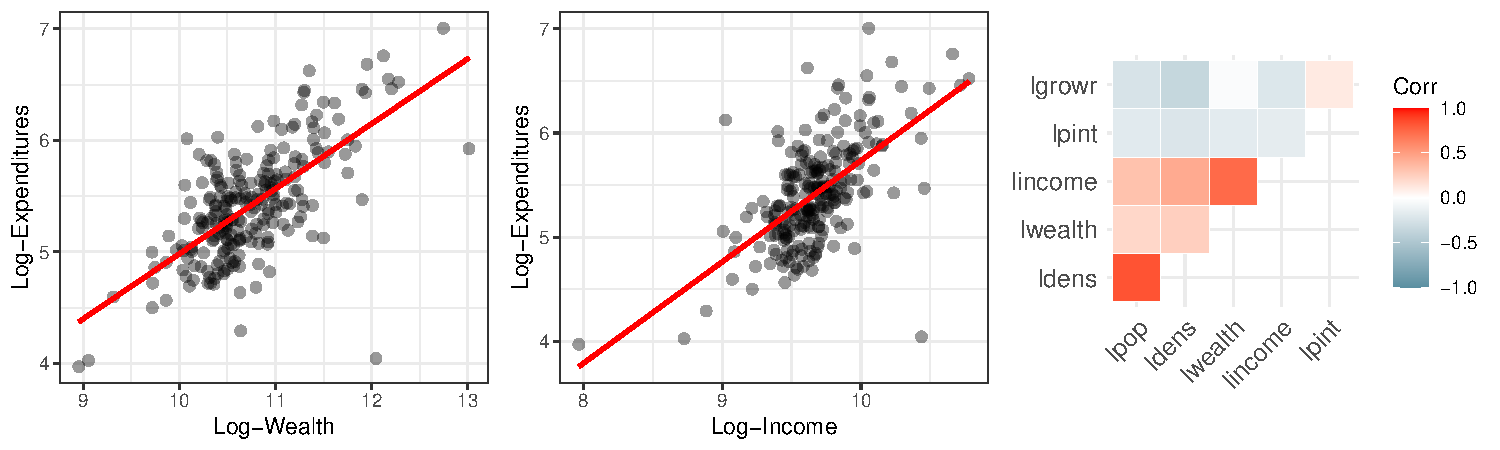
\includegraphics[width=4in]{figure/unnamed-chunk-3-1} 

\end{knitrout}

\caption{Pairwise scatterplot of variables}
\label{pairwise_scatterplot}
\end{center}
\end{figure}

% Write a short blurb citing the figure and stating what it is.
When exploring the relationship between each variable, a pairwise scatterplot was created, see Figure~\{pairwise_scatterplot}. As seen in plot, Outstate and Room Board are highly correlated. 

%% Task 6: Create an appendix of code
% Here is the LaTeX code from the online video.
% Recall that this is straight LaTeX, no knitr code chunk needed!
%  \newpage
%  \noindent \Large{{\bf Appendix B: R Code}}
%  \lstinputlisting[language=R, caption = CAPTION HERE]{CODE FILE NAME HERE}


\end{document}
